%Modified CVPR 2026 Paper Template; see https://github.com/cvpr-org/author-kit

\documentclass[10pt,twocolumn,letterpaper]{article}

%%%%%%%%% PAPER TYPE
%\usepackage{cvpr}              % To produce the CAMERA-READY version
%\usepackage[review]{cvpr}      % To produce the REVIEW version
\usepackage[pagenumbers]{cvpr} % To force page numbers, e.g. for an arXiv version

% Import additional packages in the preamble file, before hyperref
\input{preamble}

% It is strongly recommended to use hyperref, especially for the review version.
% hyperref with option pagebackref eases the reviewers' job.
% Please disable hyperref *only* if you encounter grave issues,
% e.g. with the file validation for the camera-ready version.
%
% If you comment hyperref and then uncomment it, you should delete *.aux before re-running LaTeX.
% (Or just hit 'q' on the first LaTeX run, let it finish, and you should be clear).
\definecolor{cvprblue}{rgb}{0.21,0.49,0.74}
\usepackage[pagebackref,breaklinks,colorlinks,allcolors=cvprblue]{hyperref}

\usepackage{booktabs}
\usepackage{multirow}
\usepackage{graphicx}

%%%%%%%%% PAPER ID - IGNORE THIS
\def\paperID{*****}
\def\confName{CVPR}
\def\confYear{2026}

%%%%%%%%% TITLE - PLEASE UPDATE
\title{Gipfelsturm: Maximizing LLM Training Throughput on GH200 GPUs\thanks{This work was done as part of the Large-Scale AI Engineering course of ETH Zurich.}}

%%%%%%%%% AUTHORS - PLEASE UPDATE
\author{Baudoin Coispeau
\and
Gaspard Thoral
\and
Rayane Charif Chefchaouni
}

\begin{document}
\maketitle


\section{Project Overview}
\label{sec:intro}

\textit{Gipfelsturm} (German: ``summit attempt'') targets \textbf{Challenge 2}: achieving the highest tokens/sec/GPU for a given model size on a single node (4$\times$GH200 GPUs) of the CSCS Alps supercomputer. We use Megatron-LM~\cite{shoeybi2019megatron} as the training framework and systematically explore three orthogonal optimization axes — compute kernels, precision \& memory strategies, and intra-node parallelism — before combining the best techniques into a single winning stack.

Our three-phase approach (familiarization, independent exploration, integration) lets each team member own one axis while sharing a common benchmark harness. The final configuration targets a $\sim$3B parameter model on a single GH200 node, with a stretch goal of $\sim$32B with tensor parallelism (TP=4).


\section{Implementation}
\label{sec:implementation}

\subsection{Infrastructure \& Baseline}

All training is orchestrated through a \texttt{launch.sh} script that generates self-contained SLURM batch scripts and submits them to the Clariden partition of the Swiss AI Initiative's Alps cluster. The cluster provides GH200 compute nodes (4 GPUs per node, connected via NVLink-C2C) linked by the Slingshot-11 interconnect.

We use the \textbf{alps3} container image (NGC PyTorch 26.01-py3), which includes patched NCCL 2.29.3-1, libfabric 2.5.0a1, OpenMPI 5.0.9, and nvshmem 3.4.5-0. Training data is the \textbf{Nemotron-ClimbMix} \texttt{climbmix\_small} subset ($\sim$6--12B tokens, GPT-2 BPE tokenizer), pre-converted to Megatron's binary format and stored on capstor.

The baseline model architecture follows a standard transformer with RoPE positional embeddings, GQA, SwiGLU activations, and RMSNorm — matching the configuration shipped with Megatron-LM \texttt{core\_v0.16.1}. Default training hyperparameters: sequence length 4096, global batch size 256, AdamW ($\beta_1{=}0.9$, $\beta_2{=}0.95$), weight decay 0.1, learning rate $3\times10^{-4}$, BF16 mixed precision with TransformerEngine (\texttt{--transformer-impl transformer\_engine}).

\subsection{Megatron-LM Patches}

Local modifications to the Megatron-LM submodule are managed as isolated patch files (applied automatically by \texttt{launch.sh} via \texttt{git apply}). This keeps the submodule clean and upgradeable. The first patch (\texttt{0001-log-tokens-per-sec-to-wandb.patch}) adds tokens/sec/GPU logging to stdout, TensorBoard, and W\&B inside \texttt{training\_log()}, since Megatron-LM natively only reports TFLOP/s/GPU.

\subsection{Shared Benchmark Harness}

A canonical benchmark script produces a single throughput number (tokens/sec/GPU averaged over 50 warm-up steps) for any model/configuration pair. All runs are logged to a shared W\&B project under the \texttt{gipfelsturm} experiment name, with standardized metrics: tokens/sec, MFU, GPU memory utilization, and loss. This ensures every team member's ablations are directly comparable.

\subsection{Optimization Axes}

\paragraph{Baudoin — Intra-node Parallelism.}
We sweep tensor parallelism from TP=1 to TP=4 (exploiting the 4 GH200 GPUs on a single node), with and without sequence parallelism. We also tune TP communication overlap (\texttt{--overlap-grad-reduce}, \texttt{--overlap-param-gather}) and sweep global batch size with gradient accumulation steps to identify the optimal MFU operating point.

\paragraph{Gaspard — Precision \& Memory.}
Starting from the BF16 baseline, we enable FP8 training via TransformerEngine and verify that loss curves remain aligned. We then benchmark ZeRO-1/2/3 optimizer state sharding for throughput and memory, and evaluate activation (gradient) checkpointing as a memory-capacity relief valve. Each configuration is placed on a memory–throughput Pareto chart.

\paragraph{Rayane — Compute Kernels.}
NSYS profiling identifies the dominant kernels in the baseline configuration. We then evaluate FlashAttention (\texttt{--use-flash-attn}), Liger-Kernel fused operators (RMSNorm, SwiGLU, cross-entropy), Cut Cross-Entropy, and \texttt{torch.compile}. Each optimization is measured independently and stacked, probing whether kernel-level fusion offers any headroom on top of the TransformerEngine backend.

\section{Experiments}
\label{sec:experiments}

\subsection{Experimental Setup}

All throughput measurements are performed over 50 training steps (skipping the first 2 for warm-up) at sequence length 4096 on a single GH200 node (4 GPUs). The metric reported is \textbf{tokens/sec/GPU}. Model sizes follow the configurations in Table~\ref{tab:baselines}; we focus compute-kernel exploration on the 8B model (TP=1, PP=1) to isolate kernel-level effects from parallelism overhead.

\begin{table}[h]
  \caption{Single-GPU throughput baselines (TP=1, PP=1, SEQ=4096, BF16).}
  \label{tab:baselines}
  \centering
  \small
  \begin{tabular}{@{}lcc@{}}
    \toprule
    Model & MBS & tok/s/GPU \\
    \midrule
    125M  & 16 & 54{,}671 \\
    350M  & 8  & 62{,}711 \\
    760M  & 6  & 74{,}994 \\
    1.5B  & 4  & 34{,}054 \\
    3B    & 4  & 19{,}842 \\
    8B    & 2  & 10{,}882 \\
    \bottomrule
  \end{tabular}
\end{table}

\subsection{Parallelism Sweep}

Table~\ref{tab:tp_sweep} shows the effect of tensor parallelism on the 3B model. Sequence parallelism is evaluated on top of TP=4 and the communication overlap flags are toggled independently. \TODO{Fill with actual measured numbers.}

\begin{table}[h]
  \caption{Tensor parallelism sweep on the 3B model (single GH200 node).}
  \label{tab:tp_sweep}
  \centering
  \small
  \begin{tabular}{@{}lccc@{}}
    \toprule
    Config & TP & Seq.~Par. & tok/s/GPU \\
    \midrule
    Baseline      & 1 & --   & \TODO{X} \\
    TP=2          & 2 & --   & \TODO{X} \\
    TP=4          & 4 & --   & \TODO{X} \\
    TP=4 + SP     & 4 & Yes  & \TODO{X} \\
    \bottomrule
  \end{tabular}
\end{table}

\subsection{Precision \& Memory}

Table~\ref{tab:precision} summarizes the throughput and peak GPU memory for each precision and memory strategy. \TODO{Fill with actual measured numbers.}

\begin{table}[h]
  \caption{Precision and memory strategy comparison on the 3B model.}
  \label{tab:precision}
  \centering
  \small
  \begin{tabular}{@{}lccc@{}}
    \toprule
    Config & tok/s/GPU & Mem (GB) \\
    \midrule
    BF16 (baseline)        & \TODO{X} & \TODO{X} \\
    FP8 (TransformerEngine)& \TODO{X} & \TODO{X} \\
    BF16 + ZeRO-1          & \TODO{X} & \TODO{X} \\
    BF16 + ZeRO-2          & \TODO{X} & \TODO{X} \\
    BF16 + Grad.~Ckpt.     & \TODO{X} & \TODO{X} \\
    \bottomrule
  \end{tabular}
\end{table}

\subsection{Compute Kernel Ablation}

We benchmark five kernel-level optimizations on the 8B model (TP=1, PP=1, BF16, GBS=256, SEQ=4096) using TransformerEngine as the backend. Each configuration is measured over 50 steps; Table~\ref{tab:kernels} reports the average of steps 3--50.

\begin{table}[h]
  \caption{Kernel optimization ablation (8B model, TP=1, TransformerEngine backend).}
  \label{tab:kernels}
  \centering
  \small
  \begin{tabular}{@{}lcc@{}}
    \toprule
    Config & tok/s/GPU & $\Delta$ \\
    \midrule
    Baseline (BF16 + TE)         & 11{,}051 & ---       \\
    + FlashAttention             & 10{,}726 & $-$2.9\%  \\
    + Liger RMSNorm              & 10{,}945 & $-$1.0\%  \\
    + FA + Liger RMSNorm         & 10{,}743 & $-$2.8\%  \\
    + Cut Cross-Entropy (CCE)    & 10{,}865 & $-$1.7\%  \\
    \texttt{torch.compile}       & \multicolumn{2}{c}{incompatible$^\dagger$} \\
    \bottomrule
  \end{tabular}
  \vspace{2pt}
  {\footnotesize $^\dagger$\texttt{torch.compile} raises \texttt{AssertionError} in Megatron-LM's DDP forward pre-hook (\texttt{core\_v0.16.1}).}
\end{table}

\textbf{All optimizations show neutral-to-negative impact} ($-$1\% to $-$3\%). NSYS profiling confirms the root cause: TransformerEngine occupies $\sim$99.8\% of the default CUDA stream with its own fused \texttt{nvte\_*} kernels throughout each iteration. The GPU is already saturated — there is no idle time for additional kernel fusion to exploit.

Concretely: (1)~\textbf{FlashAttention} is redundant because TE's \texttt{TEDotProductAttention} uses an equivalent fused attention path internally; adding \texttt{--use-flash-attn} on top of TE introduces a conflict that costs 2.9\%. (2)~\textbf{Liger-Kernel} v0.8.0 does not yet support \texttt{apply\_liger\_kernel\_to\_megatron} (open PR \#1207 as of May 2026); we manually patched \texttt{FusedRMSNorm} with \texttt{LigerRMSNorm}, but TE overrides the norm computation with its own fused path, rendering the patch a near no-op with $-$1\% overhead from the wrapper. (3)~\textbf{torch.compile} is incompatible with Megatron-LM's DDP hook implementation in \texttt{core\_v0.16.1}, causing an \texttt{AssertionError} on \texttt{disable\_forward\_pre\_hook()} before training begins.

\begin{figure}[h]
  \centering
  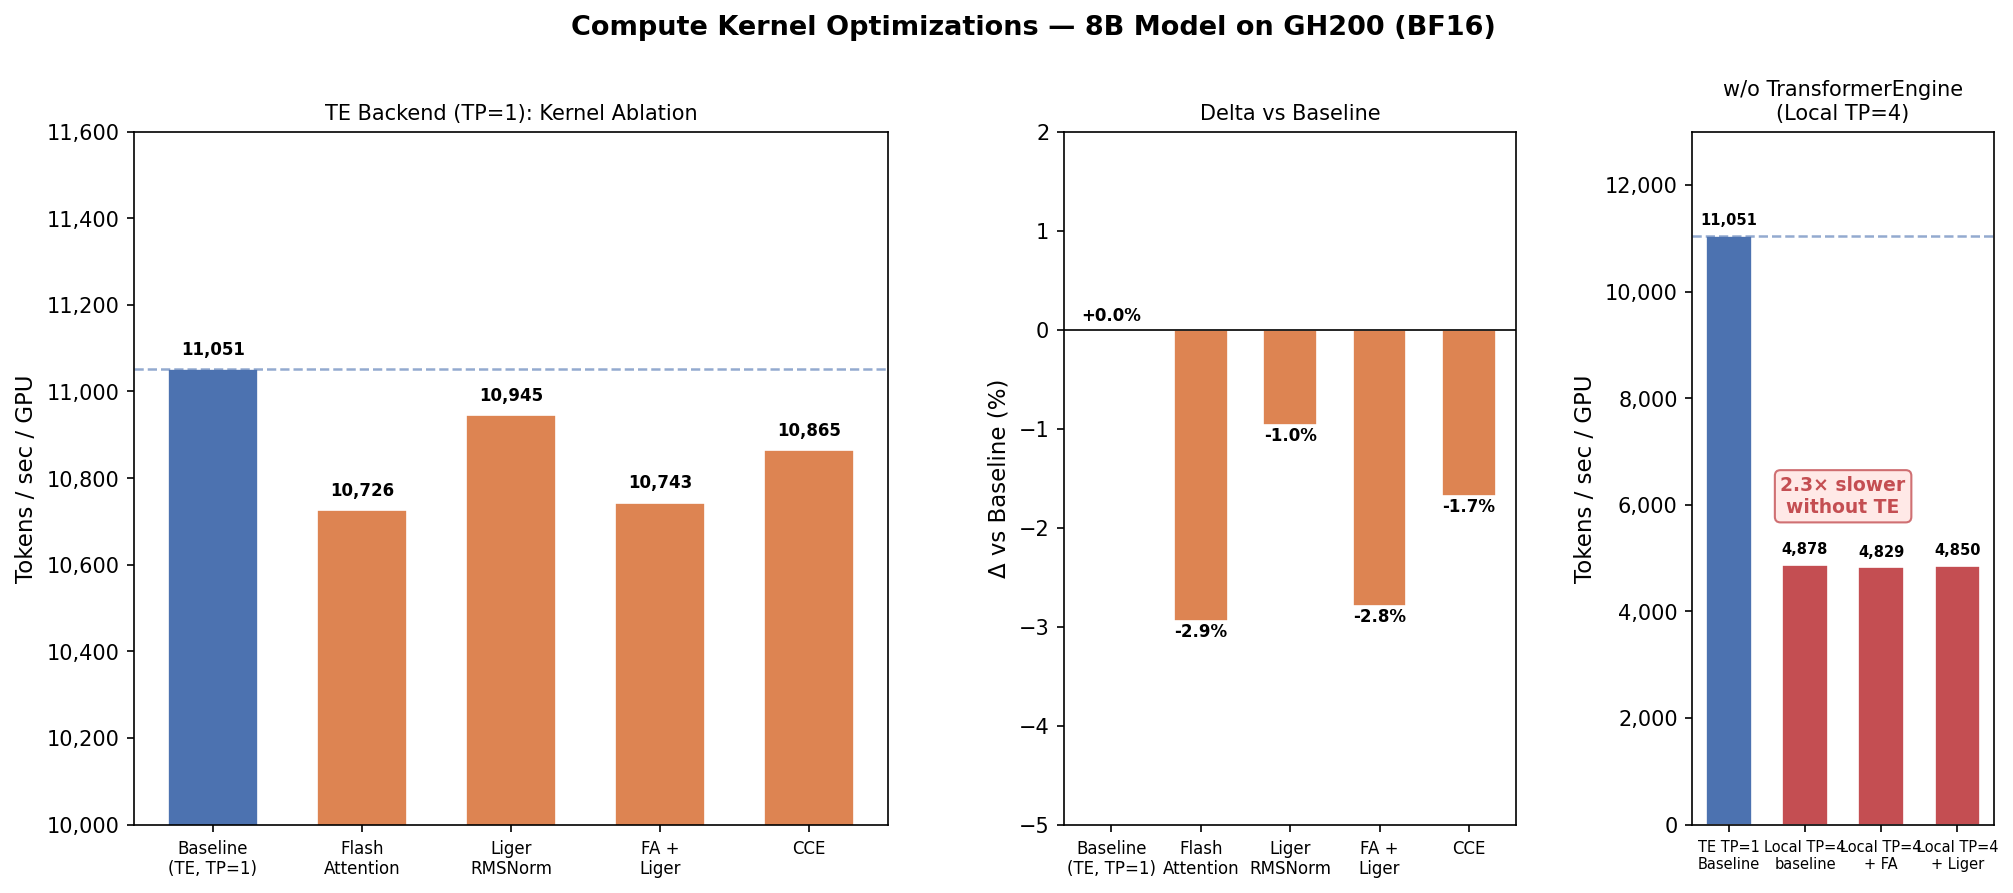
\includegraphics[width=\linewidth]{../analysis/pareto_chart.png}
  \caption{Kernel optimization Pareto on the 8B model. All techniques show neutral-to-negative impact when applied on top of the TransformerEngine backend.}
  \label{fig:pareto}
\end{figure}

\textbf{TransformerEngine is a prerequisite, not an optimization.} To quantify TE's contribution, we ran the same 8B model with \texttt{--transformer-impl local} (Megatron's native PyTorch implementation). TP=1 and TP=2 configurations failed with CUDA OOM (96\,GB GH200) — without TE's fused kernels, the O($n^2$) attention matrix and unoptimized gradient buffers exceed GPU capacity at GBS=256. Using TP=4 (which splits the model across all 4 GPUs, reducing per-GPU memory) resolves the OOM and yields measurable results: \textbf{4{,}878 tok/s/GPU}, which is $\mathbf{2.26\times}$ \textbf{slower} than the TE TP=1 baseline (11{,}051 tok/s/GPU). This 2.3$\times$ gap confirms that TransformerEngine is not an optional add-on but a hardware-level prerequisite for efficient 8B model training on GH200.


\section{Results}
\label{sec:results}

\subsection{Compatibility Matrix}

Before the final integration run, we identify which optimization pairs are safe to combine. Known compatibility issues include \texttt{torch.compile} with tensor parallelism (graph-break risk) and FP8 with Liger-Kernel (mixed quantization-aware vs. fused kernels). A full compatibility matrix will be reported in the final version.

\subsection{Winning Stack}

\TODO{Report the final combined configuration (kernel opts + precision + parallelism) and its tokens/sec/GPU result on the 3B model (TP=4, single node). Include comparison against the baseline and MFU number. For the stretch goal, report the $\sim$32B result with TP=4.}

\subsection{Discussion}

Our three-axis methodology isolates the contribution of each optimization family and identifies which combinations stack cleanly. The patch-based workflow for Megatron-LM ensures that infrastructure changes remain reviewable and upgradeable independently of the optimization code.

\textbf{Key finding from the compute-kernel axis:} on GH200 with TransformerEngine, traditional application-layer kernel optimizations (FlashAttention, Liger-Kernel, torch.compile) offer no throughput benefit. The performance ceiling is already set by TE's hardware-aware CUDA kernels, which achieve $\sim$99.8\% GPU stream utilization. Future work on this axis should target operations outside TE's scope — notably the cross-entropy loss over large vocabularies. The integration axis will clarify whether FP8 (Gaspard) and optimal TP (Baudoin) unlock headroom beyond the TE baseline. \TODO{Discuss key findings and unexpected conflicts once experiments are complete.}


\cleardoublepage
{
    \small
    \bibliographystyle{ieeenat_fullname}
    \bibliography{main}
}


\end{document}
